
In this section, we will describe the solution that we have come up with to satisfy the quality attributes that we have chosen to prioritize for this project. We will furthermore argue the tactics used to achieve the quality attribute scenarios and discuss potential trade-offs of said tactics.

The following image is a diagram of the entire system. Its parts are grouped into boxes to highlight the different sections of the system.
\begin{center}
    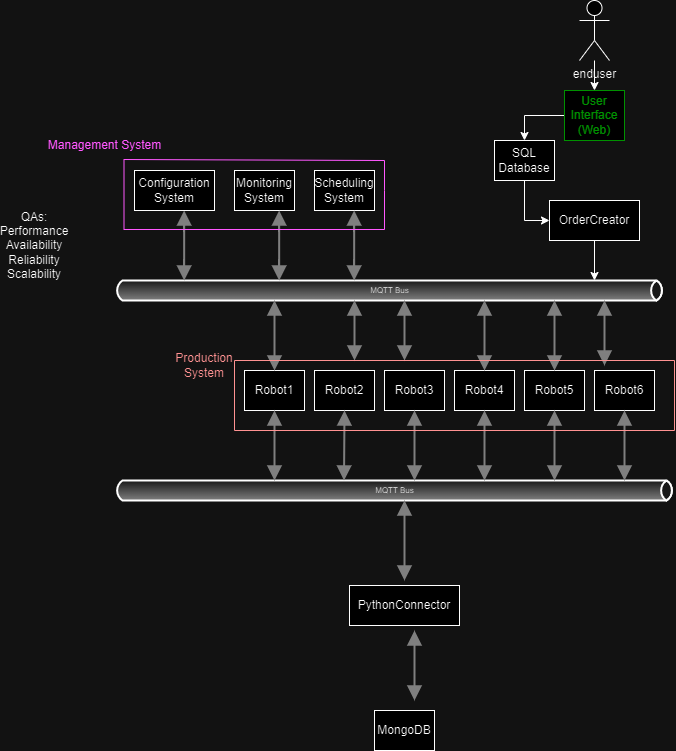
\includegraphics[scale=0.38]{Images/Systemdiagram.drawio.png}
\end{center}
\vspace{1em}

Overall we have a production system, which consists of the robots on our assembly line.
The subsystem connects to two different MQTT message buses, one for handling logging data and one for handling configuration, heartbeats, and scheduling. The idea of the two separate message buses was intentional to prevent any problems where scaling of the production line or the amount of logging entries, would result in so much logging data that it would affect other parts of the system. Therefore we chose to have an additional separate channel for logging. The allocation of an additional message bus is a tactic to increase performance, in that we have essentially increased the resources of the project or at least made the system able to scale in different contexts of use of the message busses.


Next, our management system consists of two different parts: A monitoring system and a scheduling system.

The scheduling system acts as an orchestrator in our system, as it takes orders from our "Order Creator" module, arranges system configurations, and starts the production line if there are no current ongoing processes.
Using a scheduling system to distribute our resources, is a tactic to increase performance since it allows for the possibility of introducing concurrency\cite{lenbassArchi}.

The monitoring system pings every robot on the assembly line to detect whether or not they are alive. 
This is a tactic that seeks to increase the availability of the system. This tactic is called Ping/Echo or heartbeat and is classified under the fault detection category of the availability tactics \cite{lenbassArchi}. This was one of the major things that we had to ensure were working as intended, since we want a system that is able to run 24/7. This means that in the context of robots, we have to essentially have a way to detect any errors to notify the appropriate personnel as quickly as possible in case of problems with the system. One downside to this however could be, that if the operation is scaled, then the amount of heartbeats that had to be sent out to every robot could potentially clog the MQTT message bus. This could however be solved by further increasing the resource of the system by introducing yet another MQTT bus to handle the heartbeats separately.   

Overall, the entirety of our system is dockerized and has a development pipeline in the form of GitHub actions that make the system continuously deployable. This means that if any changes are pushed to the main branch of the GitHub repository, the pipeline automatically analyses, builds, and deploys the code. This results in a framework where the developers can push small changes multiple times a day. The workflow can be seen in the section \ref{sec:github_workflow}, where it is showcased that the pipeline has some build jobs for each of the dockerfiles of the system and then a deploy job to deploy all of the created artifacts on a Google VM. This part of the system had a lot of issues but works as intended when the VM from Google is turned on.

In addition to this, the major way of communicating in the system is through the MQTT message busses, as described earlier. This provides interoperability for the system because different programming languages and frameworks can interact with each other given that they have access to the bus and are configured to use the chosen data communication format, for this project it is JSON.\cite{lenbassArchi} This encapsulates the different entities of the system and allows them to be loosely coupled, which further means that they are able to be replaced with entirely different modules, so long that they utilize the same data format for communication.

At last, we decided to address the quality attribute performance by introducing the tactic \emph{schedule resource} and \emph{manage work requests}\cite{lenbassArchi}. This was done by introducing a Scheduler module and a OrderCreate module which is responsible for managing the queue of the tanks that have been ordered but not yet produced. The idea is for the OrderCreate module to scan the PostgreSQL database to check, if there are any orders that, have not yet been delivered to our scheduling system. If so, the OrderCreate will pull the necessary data from the database to create a JSON object and publish it to a topic in our MQTT bus, which the scheduling system will then read, and when the robots are ready, it will then begin processing the new order. When the order is done, it will notify the OrderCreate module that the order has been completed, and the OrderCreate module will then update the isdone column of the order in the database. This workflow illustrates how we are scheduling resources and managing the amount of work requests in our system, which is by managing them in a queue and having flags around the system to ensure that the orders do not get stuck on their way throughout the system. 
